\begin{exercises} 

\item Consider the graph of the function $y = p(x)$ that is provided in Figure~\ref{F:1.7.Ez2}.  Assume that each portion of the graph of $p$ is a straight line, as pictured.
\begin{figure}[h]
\begin{center}
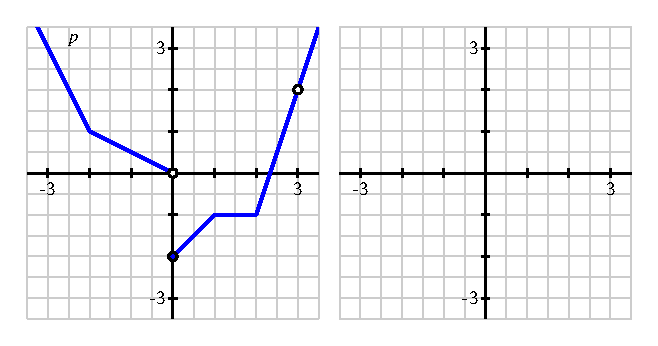
\includegraphics{figures/1_7_Ez2.eps}
\caption{At left, the piecewise linear function $y = p(x)$.  At right, axes for plotting $y = p'(x)$.} \label{F:1.7.Ez2}
\end{center}
\end{figure}
	\ba
		\item State all values of $a$ for which $\lim_{x \to a} p(x)$ does not exist.
		\item State all values of $a$ for which $p$ is not continuous at $a$.
		\item State all values of $a$ for which $p$ is not differentiable at $x = a$.
		\item On the axes provided in Figure~\ref{F:1.7.Ez2}, sketch an accurate graph of $y = p'(x)$.
	\ea

\item For each of the following prompts, give an example of a function that satisfies the stated criteria.  A formula or a graph, with reasoning, is sufficient for each.  If no such example is possible, explain why.
	\ba
	  \item A function $f$ that is continuous at $a = 2$ but not differentiable at $a = 2$.
	  \item A function $g$ that is differentiable at $a = 3$ but does not have a limit at $a=3$.
	  \item A function $h$ that has a limit at $a = -2$, is defined at $a = -2$, but is not continuous at $a = -2$.
	  \item A function $p$ that satisfies all of the following:
	  \begin{itemize}
	  	\item $p(-1) = 3$ and $\lim_{x \to -1} p(x) = 2$
		\item $p(0) = 1$ and $p'(0) = 0$
		\item $\lim_{x \to 1} p(x) = p(1)$ and $p'(1)$ does not exist
	  \end{itemize}
	\ea

\item Let $h(x)$ be a function whose derivative $y= h'(x)$ is given by the graph on the right in Figure~\ref{F:1.7.Ez3}.
	\ba
		\item Based on the graph of $y = h'(x)$, what can you say about the behavior of the function $y = h(x)$?
		\item At which values of $x$ is $y = h'(x)$ not defined?  What behavior does this lead you to expect to see in the graph of $y=h(x)$?
		\item Is it possible for $y = h(x)$ to have points where $h$ is not continuous?  Explain your answer.
		\item On the axes provided at left, sketch at least two distinct graphs that are possible functions $y = h(x)$ that each have a derivative $y = h'(x)$ that matches the provided graph at right.  Explain why there are multiple possibilities for $y = h(x)$.
	\ea
\begin{figure}[h]
  \begin{center}
 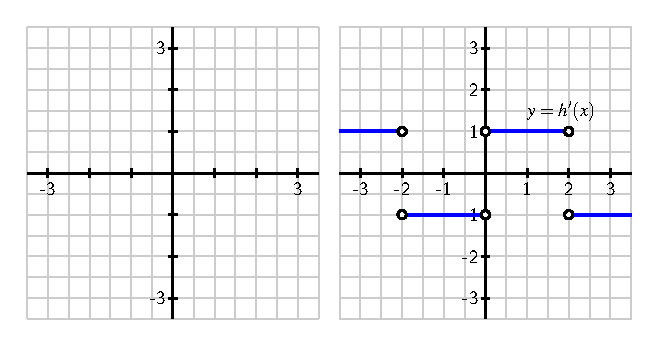
\includegraphics{figures/1_7_Ez3.eps} %\ \  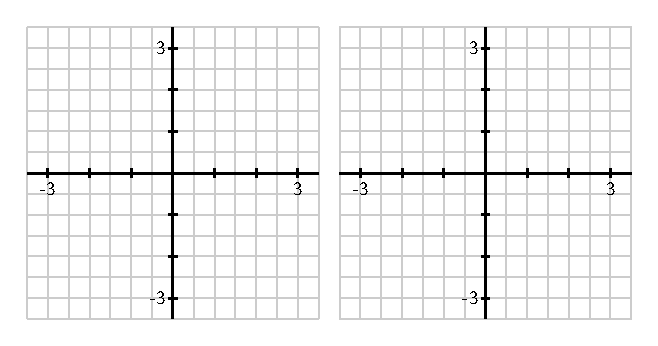
\includegraphics{figures/1_2_Ez3.eps}
   \end{center}
   \caption{Axes for plotting $y = h(x)$ and, at right, the graph of $y = h'(x)$.} \label{F:1.7.Ez3}
\end{figure}

\item Consider the function $g(x) = \sqrt{|x|}$.
	\ba
		\item Use a graph to explain visually why $g$ is not differentiable at $x = 0$.
		\item Use the limit definition of the derivative to show that
		$$g'(0) = \lim_{h \to 0} \frac{\sqrt{|h|}}{h}.$$
		\item Investigate the value of $g'(0)$ by estimating the limit in (b) using small positive and negative values of $h$.  For instance, you might compute $\frac{\sqrt{|-0.01|}}{0.01}$.  Be sure to use several different values of $h$ (both positive and negative), including ones closer to 0 than 0.01.  What do your results tell you about $g'(0)$?
		\item Use your graph in (a) to sketch an approximate graph of $y = g'(x)$.  
	\ea

\end{exercises}
\afterexercises